\documentclass{article}
\renewcommand{\thesubsection}{\thesection.\alph{subsection}}
\usepackage{graphicx} % Required for inserting images
\usepackage{listings}
\usepackage{xcolor}
\usepackage{hyperref}

\definecolor{codegreen}{rgb}{0,0.6,0}
\definecolor{codegray}{rgb}{0.5,0.5,0.5}
\definecolor{codepurple}{rgb}{0.58,0,0.82}
\definecolor{backcolour}{rgb}{0.95,0.95,0.92}

\lstdefinestyle{mystyle}{
    backgroundcolor=\color{backcolour},   
    commentstyle=\color{codegreen},
    keywordstyle=\color{magenta},
    numberstyle=\tiny\color{codegray},
    stringstyle=\color{codepurple},
    basicstyle=\ttfamily\footnotesize,
    breakatwhitespace=false,         
    breaklines=true,                 
    captionpos=b,                    
    keepspaces=true,                 
    numbers=left,                    
    numbersep=5pt,                  
    showspaces=false,                
    showstringspaces=false,
    showtabs=false,                  
    tabsize=2
}

\lstset{style=mystyle}


\title{Compulsory Assignment 1}
\author{Lars Haukland}
\date{September 2023}

\begin{document}

\maketitle
\section{Set Theory}
\subsection{$\emptyset$}
\begin{enumerate}
    \item $\emptyset$ is the empty set symbol
    \item  It is the symbol referring to the set with no elements, \{\}.
    \item Correct:
    \begin{itemize}
        \item $\emptyset = \{\}$
        \item $\emptyset \subseteq X$
    \end{itemize}
    \item Incorrect:
    \begin{itemize}
        \item $X \supseteq \emptyset$
        \item $|\emptyset| > 3$
    \end{itemize}
\end{enumerate}

\subsection{$\cup$ and $\cap$}
\begin{enumerate}
    \item $\cup$ is the symbol for Union. \\
          $\cap$ is the symbol for Intersection
    \item $\cup$ denotes the union of two sets, e.g. all elements in both sets. $A \cup B$ \\
          $\cap$ denotes the intersection of two sets, e.g. what elements exist in both sets. $A \cap B$
    \item Correct:
    \begin{itemize}
        \item $\{1,2\} \cup \emptyset = \{1,2\}$
        \item $\{1,2\} \cup \{3\} = \{1,2,3\}$
        \item $\{1,2\} \cap \emptyset = \emptyset$
        \item $\{1,2\} \cap \{2\} = \{2\}$
    \end{itemize}
    \item Incorrect:
    \begin{itemize}
        \item $\emptyset \cup \{1\} = \{\}$
        \item $\{1,2\} \cup \{1\} = \{1\}$
        \item $\{1,2\} \cap \{3\} = \{1,2,3\}$
        \item $\{1,2\} \cap \emptyset = \{1\}$
    \end{itemize}
\end{enumerate}

\subsection{$\subseteq$ and $\supseteq$}
\begin{enumerate}
    \item $\subseteq$ is the symbol for subset equal \\
          $\supseteq$ is the symbol for superset equal
    \item $\subseteq$ denotes that a set X is a subset of, or equal, to a set Y, e.g. all elements in X are also in Y. $X \subseteq Y$ \\
          $\supseteq$ denotes that a set X is a superset of, or equal, to a set Y, e.g. all elements in Y are also in X. $X \supseteq Y$
    \item Correct:
    \begin{enumerate}
        \item $\{1, 2\} \subseteq \{1, 2, 3, 4\}$
        \item $\{1\} \subseteq \{1\}$
        \item $\{1, 2, 3, 4\} \supseteq \{1, 2\}$
        \item $\{1\} \supseteq \{1\}$
    \end{enumerate}
    \item Incorrect:
    \begin{enumerate}
        \item $\{1, 2\} \subseteq \emptyset$
        \item $\{1, 2\} \subseteq \{1\}$
        \item $\emptyset \supseteq \{1\}$
        \item $\{1, 2\} \supseteq \{1, 2, 3\}$
    \end{enumerate}
\end{enumerate}

\subsection{$\subset$ and $\supset$}
\begin{enumerate}
    \item $\subset$ is the symbol for subset \\
          $\supset$ is the symbol for superset
    \item $\subset$ denotes that a set X is a subset of, or equal, to a set Y, e.g. all elements in X are also in Y. Y and X cannot be equal $X \subseteq Y$ \\
          $\supset$ denotes that a set X is a superset of, or equal, to a set Y, e.g. all elements in Y are also in X. Y and X cannot be equal $X \supseteq Y$
    \item Correct:
    \begin{enumerate}
        \item $\{1, 2\} \subset \{1, 2, 3, 4\}$
        \item $\{1\} \subset \{1, 2\}$
        \item $\{1, 2, 3, 4\} \supset \{1, 2\}$
        \item $\{1, 2\} \supset \{1\}$
    \end{enumerate}
    \item Incorrect:
    \begin{enumerate}
        \item $\{1, 2\} \subset \emptyset$
        \item $\{1, 2\} \subset \{1, 2\}$
        \item $\emptyset \supset \{1\}$
        \item $\{1, 2\} \supset \{1, 2\}$
    \end{enumerate}
\end{enumerate}

\subsection{$\in$ and $\notin$}
\begin{enumerate}
    \item $\in$ is the symbol for "is member of" \\ $\notin$ is the symbol for "is not member of"
    \item $ a \in B$ means that an element a is a member of the set B, a exists in B \\ $a \notin B$ means that an element a is not a member of the set B, a does not exist in B
    \item Correct:
    \begin{enumerate}
        \item $1 \in \{1, 2, 3\}$
        \item $1, 4 \in \{1,2,3,4\}$
        \item $1 \notin \{2,3,4\}$
        \item $1,2 \notin \emptyset$
    \end{enumerate}
    \item Incorrect:
    \begin{enumerate}
        \item $1 \in \emptyset$
        \item $2 \in \{1,3,4\}$
        \item $1 \notin \{1,2,3\}$
        \item $1,2 \notin \{1,2,3,4,5\}$
    \end{enumerate}
\end{enumerate}

\subsection{$\backslash$}
\begin{enumerate}
    \item $\backslash$ is the symbol for set-difference
    \item $X \backslash Y$ denotes everything in set X that does not occur in set Y
    \item Correct:
    \begin{enumerate}
        \item $\{1, 2\} \  \backslash \  \{1\} = \{2\}$
        \item $\{1, 2, 3\} \  \backslash \  \emptyset = \{1, 2, 3\}$
    \end{enumerate}
    \item Incorrect:
    \begin{enumerate}
        \item $\{2, 3\} \  \backslash \  \{1\} = \{1, 2, 3\}$
        \item $\emptyset \  \backslash \  \{1\} = \{1\}$
    \end{enumerate}
\end{enumerate}

\subsection{$| \ |$}
\begin{enumerate}
    \item $| \  |$ is the symbol for cardinality
    \item $|A|$ denotes the cardinality of the set A. In essence this can be viewed as size or number of things in the set. If there is a set B within the set A, this set B will be counted as 1 and not |B|.
    \item Correct: \\ Let $A = \{1,2,3\}$, $B = \{1,2\{1,2,3\}\}$
    \begin{enumerate}
        \item $|B| = 3$
        \item $|A \cup B| = 4$
    \end{enumerate}
    \item Incorrect: \\ Use same sets as previous
    \begin{enumerate}
        \item $|B| = 5$
        \item $|A \cap B| = 5$
    \end{enumerate}
\end{enumerate}


\section{Python random integer}
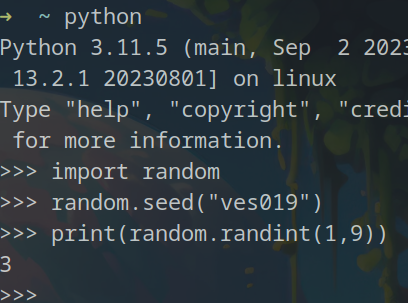
\includegraphics[scale=0.5]
{pythonRandInt.png}

\section{Algorithms}
As you can see from the previous section I got task 3 which says:\\
3. Strongly connected components\\
Give Python code computing the set of SCCs for a connected directed graph. The output should be a list of lists, each list containing an SCC. \\The function should have a docstring explaining expected input and output.
Give a convincing argument of correctness.\\
\\
To start, here is my implementation of the tarjans algorithm.
\lstinputlisting[language=Python]
{tarjans.py}
Note that the code may seem like alot but in reality it is only about 50 lines. Its just the docstrings that take up a lot of space.

\subsection{What is tarjans?}
Tarjans algorithm is an algorithm made by Robert Tarjan. It is an algorithm that finds the strongly connected components in a directed graph and runs in linear time. It is similar to Kosarajus algorithm but where Kosajarus runs in $\Theta(V+E)$, tarjans runs in $\mathcal{O}(V+E)$. \\ \\
Tarjans is basically dfs with some extra constant time operations. It starts out by looping through all the vertices in the graph. If the vertex u has not been visited (id[u] = None) then we run dfs on it.\\
The dfs marks u as visited, appends it to the stack and sets the low value. It then looks at the low of the neighbouring vertices of u. For each neighbour, if they are not yet visited then we run dfs on the neighbour and then take the minimum of the low value of u and the neighbour and assign it as the low of u, if the neighbour has been visited then we just take the min of the low values. \\
Why do we use this lows array? Say we have a vertex u with the low value lows[u] = ids[u], this is the starting low value of u as we can see in lines 94 and 95. The low value represents the index of the lowest vertex that u can reach by traversal through its neighbours. This comes in handy in the tarjans algorithm because in the end the all vertices that have the same value in the lows dictionary will be in the same strongly connected component. Here is how the algorithm runs:
\begin{enumerate}
    \item Start dfs on vertex v
    \item Loop through neighbours of v
    \begin{enumerate}
        \item If neighbour u has not been visited, then run dfs recursively on u. And then assign lows[v] = min(lows[v], lows[u]) \\
        This makes it so that if u is connected to a lower indexed vertex then we know that since v is connected to u, v is also in that component.
        \item If neighbour u has been visited, but is on the stack, e.g. a back-edge. Then we assign lows[v] = min(lows[v], ids[u]).\\
        For more details on exactly why it is ids and not lows, see \href{https://www.geeksforgeeks.org/tarjan-algorithm-find-strongly-connected-components/}{Geeks for geeks}.
    \end{enumerate}
    \item Then if the id of v and low of v are equal, we know that a new SCC is created and all vertices on the stack belong to that SCC
    \item Add all the vertices on the stack to the SCC until we reach vertex v. Add SCC list to the list of all SCCs.
\end{enumerate}

\subsection{Runtime analysys}

Firstly we have the initializing the data structures, the dictionaries ids, lows and onstack. (lines 55 - 58). This step is $\mathcal{O}(V)$. Because we have V many vertices and since a dictionary in python is a hashtable then updating keys and inserting is $\mathcal{O}(1)$.\\
Then the for loop in find\_scc\_tarjans, line 74, just makes sure that each vertex is ran dfs on. This does not change the runtime as the dfs runtime assumes that it visits every vertex.
\\
Now, as is well known the runtime of dfs is $\mathcal{O}(V + E)$. Now pseudocode for dfs can be expressed like:
\begin{lstlisting}
    DFS(G, u)
    u.visited = true
    for each v in G.Adj[u]
        if v.visited == false
            DFS(G,v)
\end{lstlisting}

Source: \hyperlink{Programiz}{https://www.programiz.com/dsa/graph-dfs}\\
If we squint our eyes, a lot, it can sort of look like the implementation of tarjans just a bit fewer steps. And that is exactly the point. We can observe that the for loop on line 101 is essentially the same as in dfs pseudocode, with the exception of hashtable operations that are $\mathcal{O}(1)$. This makes the runtime $\mathcal{O}(V+E)$.\\
Then the operations previous are in constant time as we append to our "stack" (python list), add 1 to index and change the dictionaries. All these operations are  $\mathcal{O}(1)$ and do not change the runtime.\\
Then we have this while loop. Luckily this is surrounded by an if statement making sure that this loop goes through each SCC exactly once. In the worst case, we might have one SCC per vertex (an isolated vertex), so we can think of it as another O(V) operation. And $\mathcal{O}(2V + E)$ is equivalent to $\mathcal{O}(V+E)$

\end{document}
